\documentclass[border=4pt]{standalone}

\usepackage{amsmath}
\usepackage{tikz}
\usepackage{mathdots}
\usepackage{yhmath}
\usepackage{cancel}
\usepackage{color}
\usepackage{siunitx}
\usepackage{array}
\usepackage{multirow}
\usepackage{amssymb}
\usepackage{gensymb}
\usepackage{tabularx}
\usepackage{booktabs}
\usetikzlibrary{fadings}
\usetikzlibrary{patterns}


\begin{document}
 
 \tikzset{every picture/.style={line width=0.75pt}} %set default line width to 0.75pt

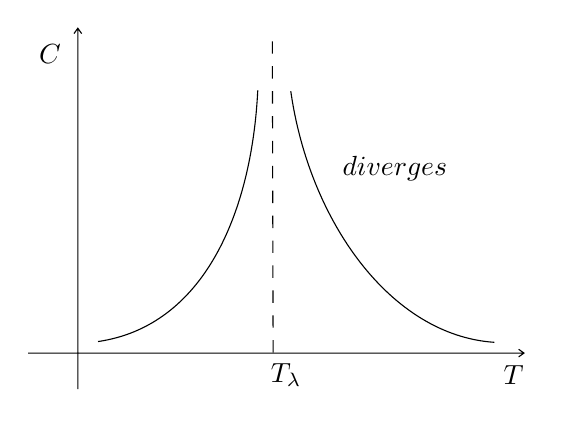
\begin{tikzpicture}[x=0.75pt,y=0.75pt,yscale=-0.37,xscale=0.37]
%uncomment if require: \path (0,476); %set diagram left start at 0, and has height of 476

%Shape: Axis 2D [id:dp5951100625553807]
\draw  (12.61,425) -- (658.18,425)(77.17,2) -- (77.17,472) (651.18,420) -- (658.18,425) -- (651.18,430) (72.17,9) -- (77.17,2) -- (82.17,9)  ;
%Straight Lines [id:da5293875835625754]
\draw  [dash pattern={on 4.5pt off 4.5pt}]  (330.5,19) -- (331.5,425) ;


%Curve Lines [id:da44190238222280653]
\draw    (103.5,410) .. controls (240.5,390) and (303.5,244) .. (311.5,83) ;


%Curve Lines [id:da7750908509461275]
\draw    (619.5,411) .. controls (484.5,402) and (378.5,253) .. (354.5,84) ;



% Text Node
\draw (644.64,453.88) node [scale=1]  {$T$};
% Text Node
\draw (348.49,453.88) node [scale=1]  {$T_{\lambda }$};
% Text Node
\draw (41,36) node [scale=1]  {$C$};
\draw (490,185) node [scale=1]  {$diverges$};

\end{tikzpicture}


\end{document}
